We also tried an approach based on TF/IDF to select which paragraphs from the news articles better summarize a sentiment shift. TF/IDF is a widely used statistic in NLP and is indeed a effective technique to extract keywords from documents. In our implementation, each news article is a list of \emph{newline-separated paragraphs}, but this can be generalized by trying every possible set of $n$ contiguous sentences in the text.
\\
Given a topic $T$, let $Tweets_T$ and $News_T$ be, respectively, the set of all the tweets and all the news articles about that topic. Then, given a shift $S$, let $Tweets_{T,S}$ and $News_{T,S}$ be the tweets and the news falling inside that contradiction window. Before applying our methodology, every document is preprocessed, in order to remove stopwords, punctuation and URLs.
\\
First, given a shift $S$, a set of $k$ keywords is computed according to their TF/IDF value w.r.t. $Tweets_T$. Then, for each paragraph, a score is calculated as the sum of the TF/IDF value of the keywords that are contained in it, divided by the length of the paragraph. Finally, for each shift, the top $p$ paragraphs are returned as a summary.
\\\\
\begin{algorithmic}
\STATE \textbf{TF/IDF Method}($T$,$k$,$p$)
\STATE
\FORALL {$S \in Shifts_T$}
	\FORALL {$word \in Tweets_{T,S}$}
		\STATE $n$ $\leftarrow$ number of total occurrences of $word$ in $Tweets_{T,S}$
		\STATE $W_{score}(word)$ $\leftarrow$ $TFIDF(word,Tweets_T) * n$
	\ENDFOR
	\STATE
	\STATE $Keywords$ $\leftarrow$ the $k$ words with highest $W_{score}$
	\STATE
	\FORALL { $Article \in News_{T,S}$ }
		\FORALL { $Paragraph \in Article$ }
			\STATE $P_{score}(Paragraph)$ $\leftarrow$ $0$

			\FORALL { $word \in Paragraph$ }
				\IF { $word \in Keywords$ }
					\STATE $P_{score}(Paragraph)$ += $W_{score}(word)$
				\ENDIF
			\ENDFOR
			\STATE $P_{score}(Paragraph)$ $\leftarrow$ ${P_{score}(Paragraph) \over |Paragraph|}$
		\ENDFOR
	\ENDFOR
	\STATE
	\STATE $summaries$($S$) $\leftarrow$ The $p$ paragraphs with highest $P_{score}$
\ENDFOR
\STATE
\RETURN $summaries$

Figure \ref{fig:TFIDF} is a graphical representation of the algorithm.

\begin{figure}[htbp]
	\centering
			{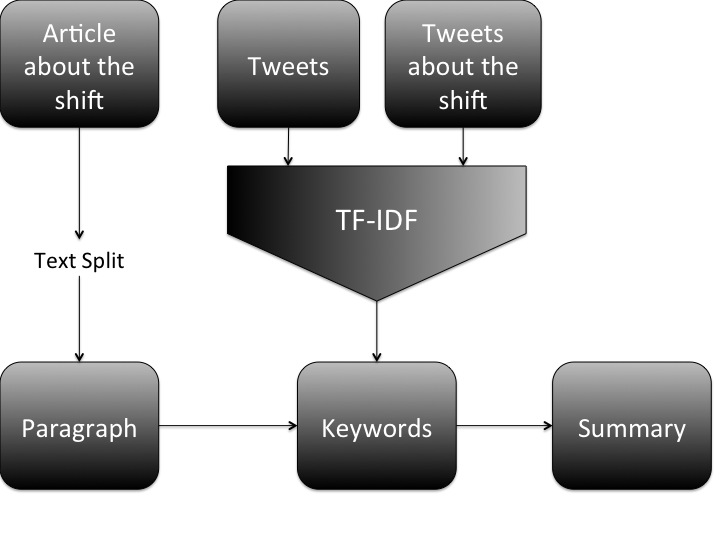
\includegraphics[width=8.5cm,height=7cm]{image/TF-IDF.jpg}}	
		\caption[TFIDF]{Graphical representation of TF/IDF algorithm}
	\label{fig:TFIDF}
\end{figure} 

\end{algorithmic}